\documentclass[dvipdfmx,autodetect-engine]{jsarticle}
\usepackage[dvipdfm]{graphicx}
\usepackage{ascmac}
\usepackage{fancybox}
\usepackage{listings}
\usepackage{plistings}
\usepackage{itembkbx}
\usepackage{amsmath}
\usepackage{url}
\usepackage{graphics}
\usepackage{listings}
\usepackage{here}

\lstset{
  basicstyle={\ttfamily},
  identifierstyle={\small},
  commentstyle={\smallitshape},
  keywordstyle={\small\bfseries},
  ndkeywordstyle={\small},
  stringstyle={\small\ttfamily},
  frame={tb},
  breaklines=true,
  columns=[l]{fullflexible},
  numbers=left,
  xrightmargin=0zw,
  xleftmargin=3zw,
  numberstyle={\scriptsize},
  stepnumber=1,
  numbersep=1zw,
  lineskip=-0.5ex
}

\textheight=23cm
\renewcommand{\figurename}{図}
\renewcommand{\tablename}{表}
\newenvironment{code}
{\vspace{0.5zw}\VerbatimEnvironment
\begin{screen} 
\baselineskip=1.0\normalbaselineskip
 \begin{Verbatim}}
{\end{Verbatim}
\baselineskip=\normalbaselineskip
 \end{screen}\vspace{0.5zw}} 

 \title{Process Monitorを用いたRAT型マルウェアの動的解析} 
 \author{山下恭平、塚本覇虎、奥若菜}
 \date{2022年6月14日}
 \begin{document} 
 \maketitle

\section{テーマ}
プロセスのログ解析によるマルウェアの検出を目標に、RAT型擬似マルウェアツールShinoBotと
監視ツールProcess Monitorを用いたマルウェアの動的解析を行う。\\

\section{環境}
本実験は以下の県境において実験を行う。
\begin{quote}
  \begin{itemize}
   \item Virtual Box ・・・ 仮想環境、今回はWindows10をインストールしている。
   \item Prosess Monitor ・・・ 動作しているプロセスを監視し、そのログを採取するソフト。
   \item ShinoBot ・・・        RAT(Random Access Tool)型のマルウェアを再現したソフト、web上に設置されたサーバから感染PCを操作できる。
  \end{itemize}
 \end{quote}

\section{実験}
\subsection{実験の概要}
ShinoBotから感染PCに命令を送り、特定のァイルを削除した時のプロセスのログと、
コマンドプロンプトから直接ファイルを削除したときのプロセスのログを取り、双方のログを比較しながら、RAT型マルウェアに見られる振る舞いを調査した。\\


\subsection{プロセスの比較}
図1、2にそれぞれ、ShinoBOTを用いてファイル削除を行なったときと、通常操作でファイルを削除したときの、プロセスの親子関係と採取されたログの量を示した。
ShinoBOTを用いる場合、ShinoBOTの実行ファイルが起動しているPCに遠隔から命令を送ると、ShinoBOTがコマンドプロンプト(cmd)を呼び出す。次に、コマンドプロンプトはConhostを呼び出す。
Conhostは外部からコマンドプロンプトを実行する際に用いられる実行ファイルである。その後、コマンドプロンプトがpowershellを呼び出し、powershellが実際にファイル削除を行う。
一方、通常操作の場合、ユーザーがコマンドプロンプトを起動させ、命令コマンドを直接打ち込まれる。その際、コマンドプロンプトによってまずconhostが呼び出されるが、conhostは何の動作も行わなかった。その後は、ShinoBotの場合と同じくpewershellが起動され、ファイルが削除された。
pewershellのログの量や内容から、どちらの場合も削除自体のプロセスにほとんど違いがないことがわかった。\\\\

\begin{figure}[H]
  \centering
  \fbox{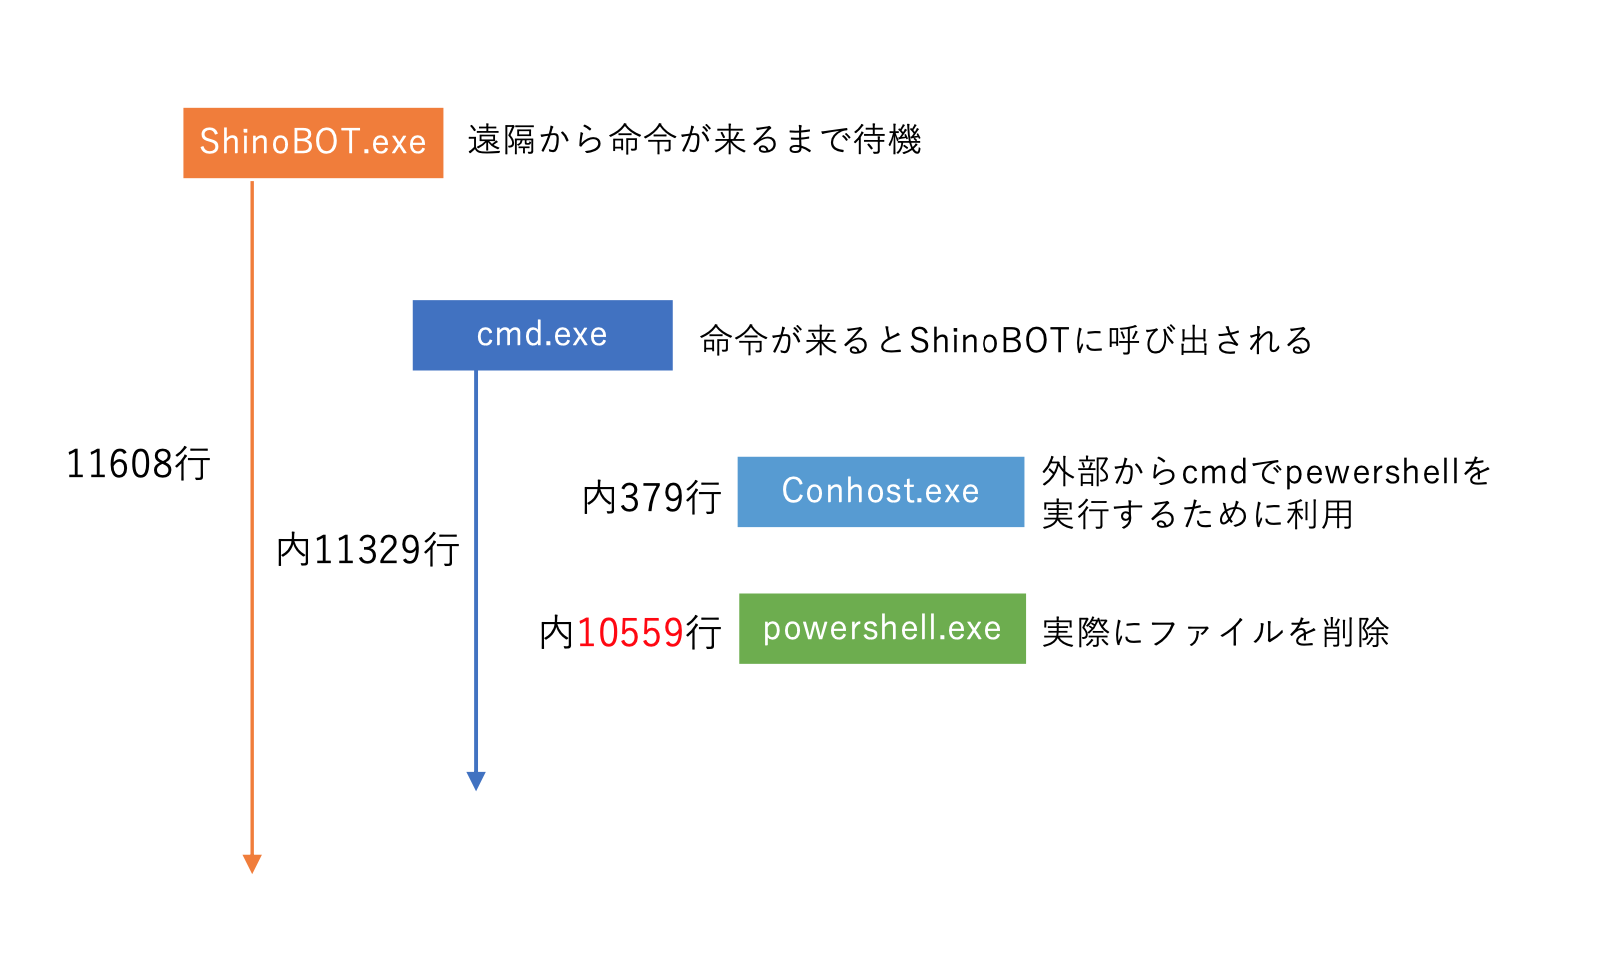
\includegraphics[scale=0.35]{shino.png}}
  \caption{}
\end{figure}

\begin{figure}[H]
  \centering
  \fbox{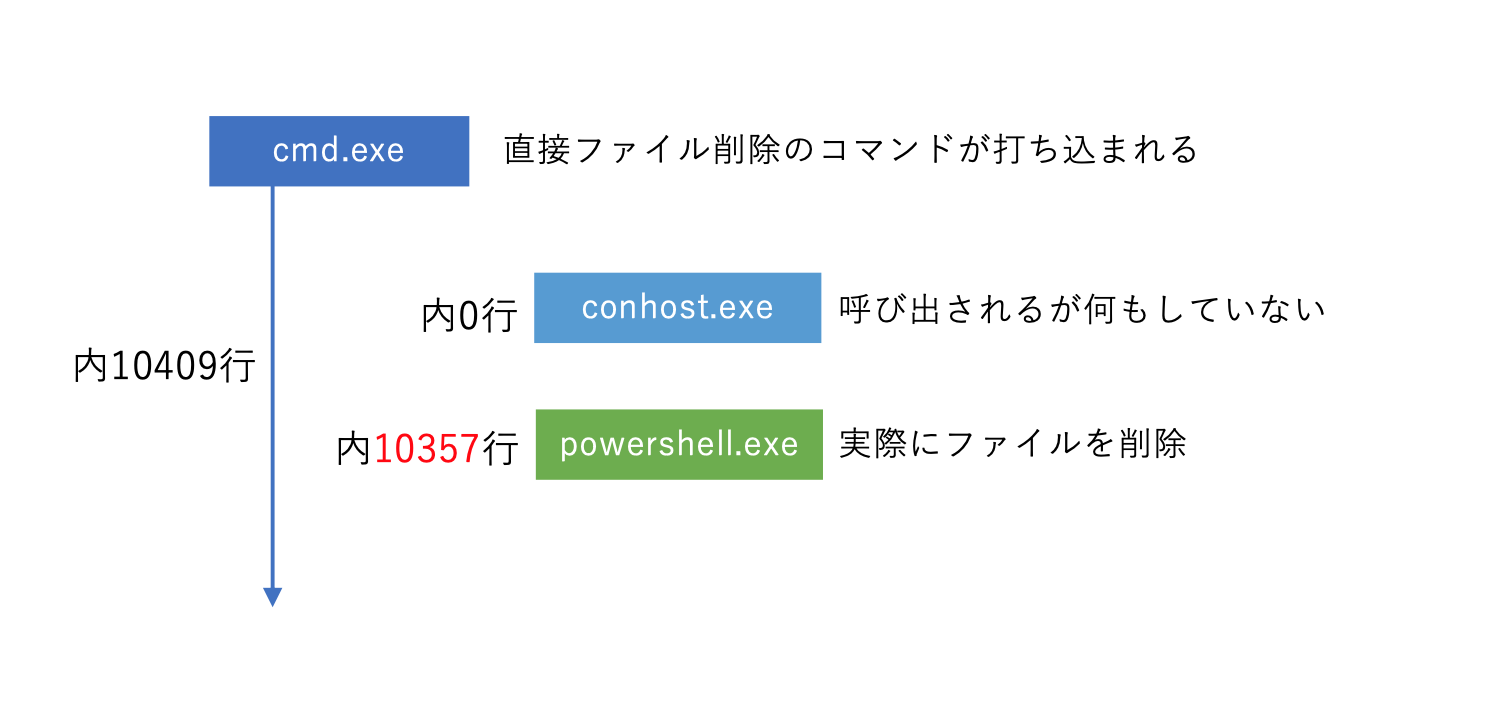
\includegraphics[scale=0.38]{normal.png}}
  \caption{}
\end{figure}

\subsection{用いられたAPIの比較}

比較を行ったそれぞれのプロセスにおいて、実際にファイルの削除を行なっていた
APIを確認したところ、同一のAPIが利用されていることが確認できた。以下は
そのAPIの詳細を示したものである。

\begin{figure}[H]
  \centering
  \fbox{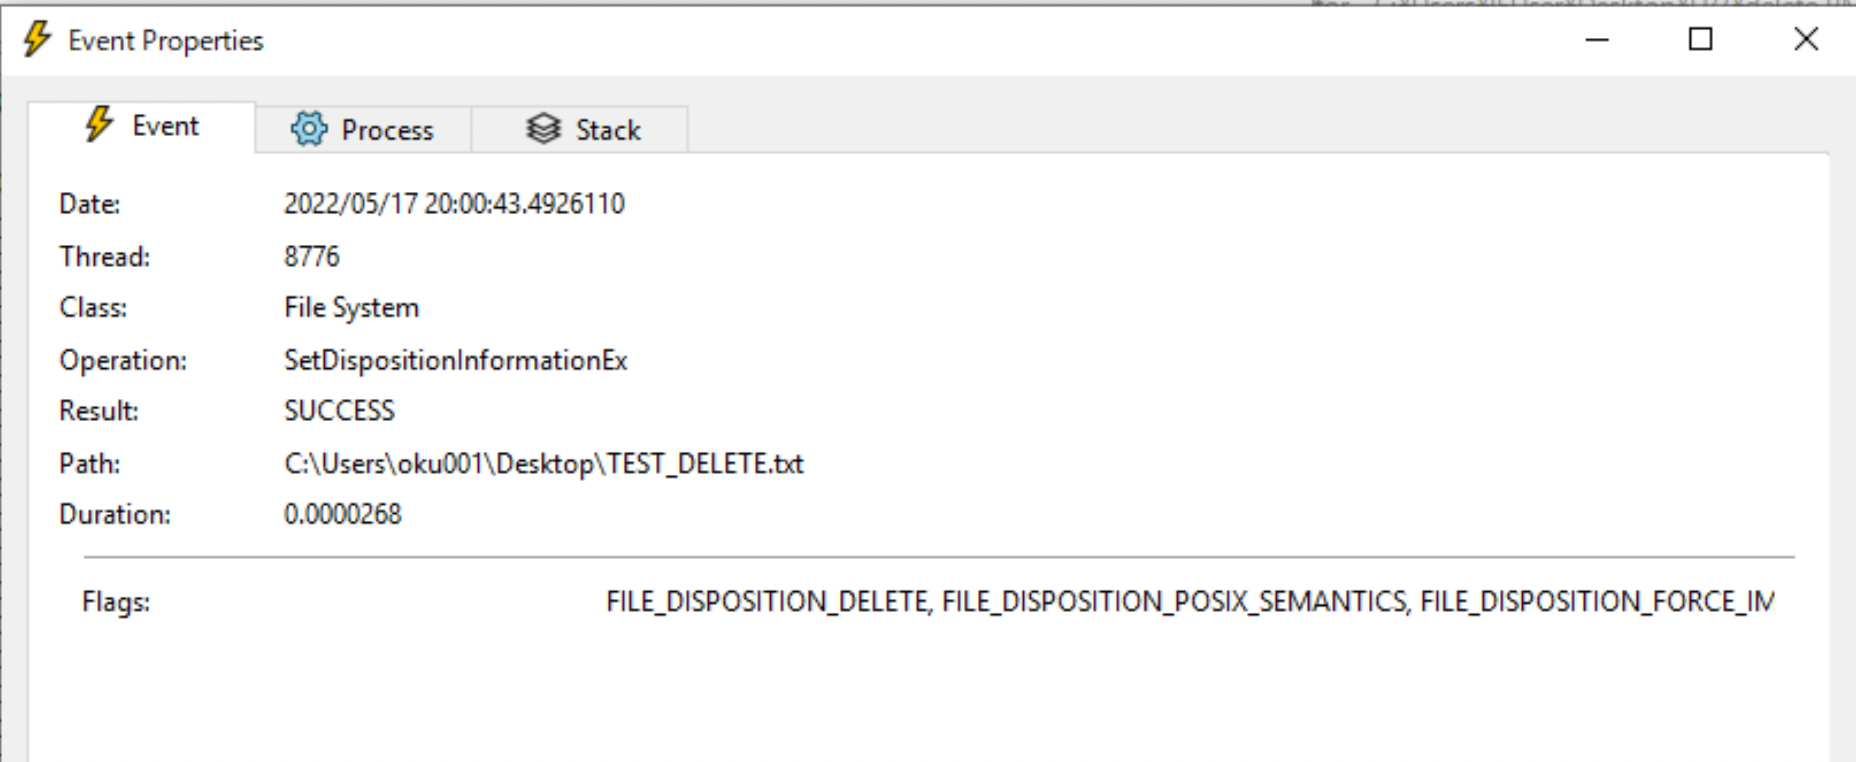
\includegraphics[scale=0.4]{pic.png}}
  \caption{}
\end{figure}

このAPIはマイクロソフトの公式ドキュメントにて、内容が公開されていたので、
その内容を記載する。\begin{math}
  ^{(1)}\end{math}

\begin{lstlisting}[caption=C++]

  typedef struct _FILE_DISPOSITION_INFORMATION_EX {
    ULONG Flags;
  } FILE_DISPOSITION_INFORMATION_EX, *PFILE_DISPOSITION_INFORMATION_EX;

\end{lstlisting}

\begin{table}[h]
  \centering
  \begin{tabular}{|ll|}
  \hline
  \textbf{フラグ名}                                   & \textbf{意味}                                                                         \\ \hline
  FILE\_DISPOSITION\_DO\_NOT\_DELETE              & \begin{tabular}[c]{@{}l@{}}システムがファイルを削除しないよう\\ に指定します。\end{tabular}                 \\ \hline
  FILE\_DISPOSITION\_DELETE                       & \begin{tabular}[c]{@{}l@{}}システムがファイルを削除することを\\ 指定します。\end{tabular}                  \\ \hline
  FILE\_DISPOSITION\_POSIX\_SEMANTICS             & \begin{tabular}[c]{@{}l@{}}システムが POSIX スタイルの削除を実\\ 行する必要があることを指定します。\end{tabular}   \\ \hline
  FILE\_DISPOSITION\_FORCE\_IMAGE\_SECTION\_CHECK & \begin{tabular}[c]{@{}l@{}}システムがイメージセクションのチェ\\ ックを強制的に実行するように指定し\\ ます。\end{tabular} \\ \hline
  FILE\_DISPOSITION\_ON\_CLOSE                    & \begin{tabular}[c]{@{}l@{}}システムが終了時の状態を設定または\\ クリアするかどうかを指定します。\end{tabular}        \\ \hline
  FILE\_DISPOSITION\_IGNORE\_READONLY\_ATTRIBUTE  & \begin{tabular}[c]{@{}l@{}}読み取り専用ファイルの削除を許可し\\ ます。\end{tabular}                     \\ \hline
  \end{tabular}
  \caption{}
  \end{table}


\subsection{通信の観測}

\begin{figure}[H]
  \centering
  \fbox{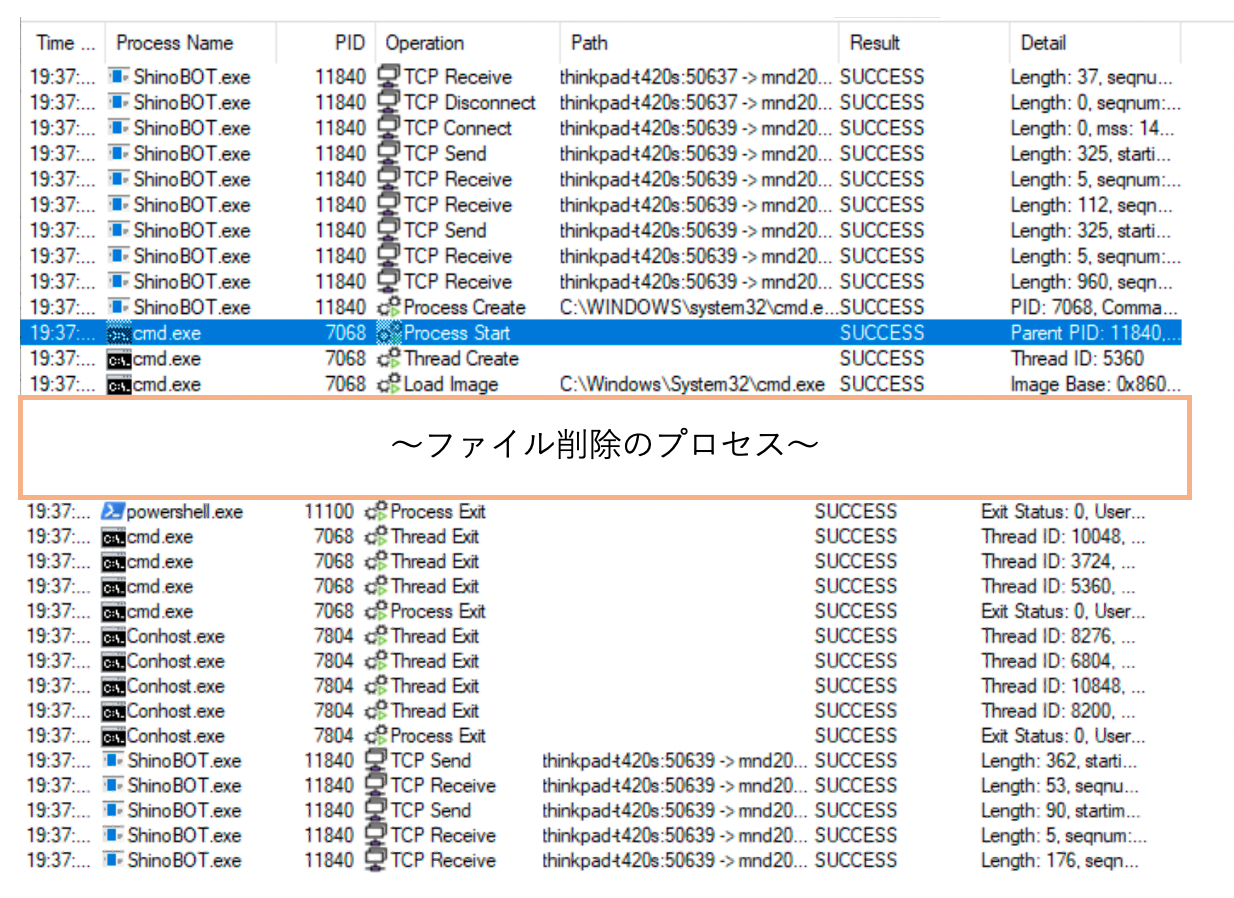
\includegraphics[scale=0.6]{tcp.png}}
  \caption{}
\end{figure}

\section{考察}
削除におけるプロセスの大部分が一位している点、用いられるAPIが通常のプロセス
と一致している点などを考慮すると。削除を行う一連のプロセス内にマルウェアだと
特徴づけるプロセスは存在しないと考えられる。この時、通信ログに着目すると削除のプロセスが
生成される前と、一連のプロセスが終了した後に、ShinoBotがTCP通信を行なっている
ことが確認できる。RATに感染しているコンピュータはサーバから送られてくる命令を
実行するので、前後の通信によって、命令の受信、命令結果の送信を行なっていると
考えらる。RATに感染したコンピュータから、RATを検出する方法として、通信ログの
確認が有効な手段だと考えられる

\end{document}